\documentclass{standalone}
\usepackage{tikz, amssymb, amsmath, amsfonts}
\usetikzlibrary{arrows.meta}
\newcommand{\vect}[1]{\boldsymbol{\mathbf{#1}}}
\begin{document}
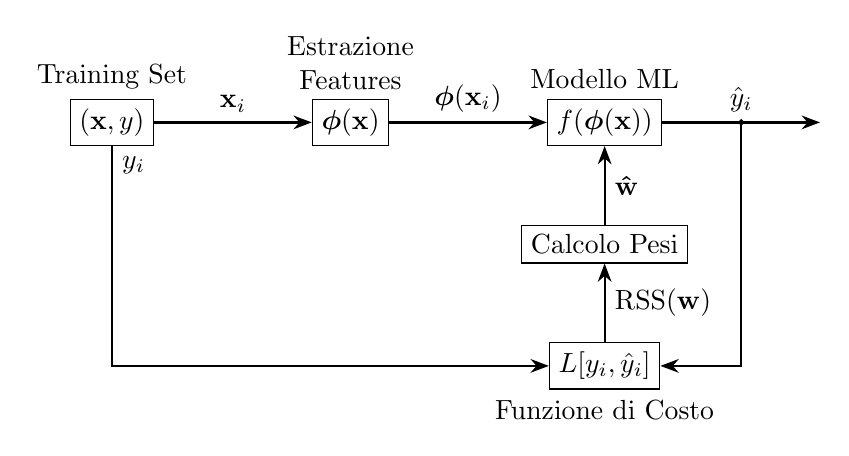
\begin{tikzpicture}
    \draw
    (0,0)node[thin, draw, rectangle, anchor=180, label={Training Set}](ts){$(\vect{x},y)$}
    [-Stealth,thick](ts.0)--++(2,0)node[midway, above]{$\vect{x}_i$}node[thin, draw, rectangle, anchor=180](p){$\vect{\phi}(\vect{x})$};
    \draw(p.90)node[above, align=center]{Estrazione\\Features};
    \draw[-Stealth,thick](p.0)--++(2,0)node[midway, above]{$\vect{\phi}({\vect{x}_i})$}node[thin, draw, rectangle, anchor=180, label={Modello ML}](ml){$f(\vect{\phi}(\vect{x}))$};
    \draw[-Stealth,thick](ml.0)--++(1,0)node[draw, circle, fill=black, inner sep=0.5pt]{}node[above]{$\hat{y}_i$}--++(1,0);
    \draw[Stealth-,thick](ml.270)--++(0,-1)node[midway, right]{$\vect{\hat{w}}$}node[thin, draw, rectangle, anchor=90](p){Calcolo Pesi};
    \draw[Stealth-,thick](p.270)--++(0,-1)node[midway, right]{RSS$(\vect{w})$}node[thin, draw, rectangle, anchor=90,label=below:{Funzione di Costo}](p){$L[y_i,\hat{y}_i]$};
    \draw[-Stealth,thick](ml.0)++(1,0)|-(p.0);
    \draw[-Stealth,thick](ts.270)node[below right]{$y_i$}|-(p.180);
\end{tikzpicture}
\end{document}